\begin{frame}[allowframebreaks]{}
    \LARGE Normalizing Flow Models: \\[1.5ex] \textbf{Coupling layers}
\end{frame}

\begin{frame}[allowframebreaks]{Coupling layers}
\textbf{Concept:}

\begin{itemize}
    \item Split the input $\mathbf{x}$ into two parts: $\mathbf{x} = [\mathbf{x}_1, \mathbf{x}_2]$.
    \item Apply a transformation to one part conditioned on the other:
    \begin{align*}
        \mathbf{y}_1 &= \mathbf{x}_1 \\
        \mathbf{y}_2 &= \mathbf{x}_2 \odot \exp\big(s(\mathbf{x}_1)\big) + t(\mathbf{x}_1)
    \end{align*}
    where $s$ and $t$ are scale and translation functions, respectively.
\end{itemize}

\textbf{Advantages:}
\begin{itemize}
    \item Invertibility is straightforward.
    \item The Jacobian is triangular, making determinant computation efficient.
    \item Facilitates the design of complex, yet tractable, transformations.
\end{itemize}
\begin{figure}
    \centering
    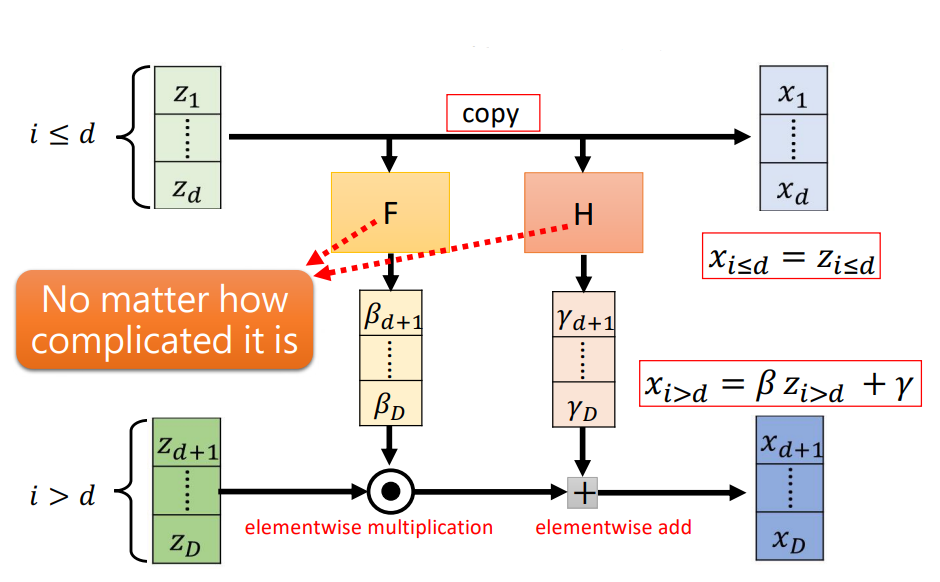
\includegraphics[height=0.9\textheight, width=\textwidth, keepaspectratio]{images/norm-flow/coupling_layer_1.png}
\end{figure}

\framebreak

\begin{figure}
    \centering
    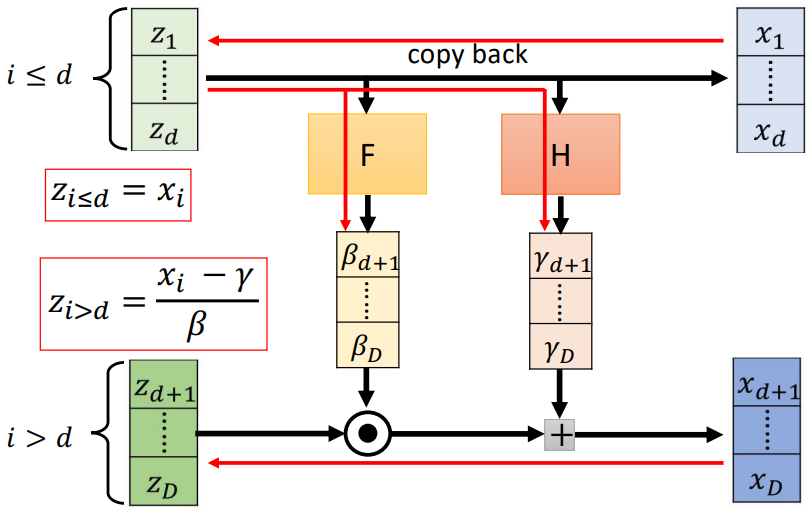
\includegraphics[height=0.9\textheight, width=\textwidth, keepaspectratio]{images/norm-flow/coupling_layer_2.png}
\end{figure}

\framebreak

\begin{figure}
    \centering
    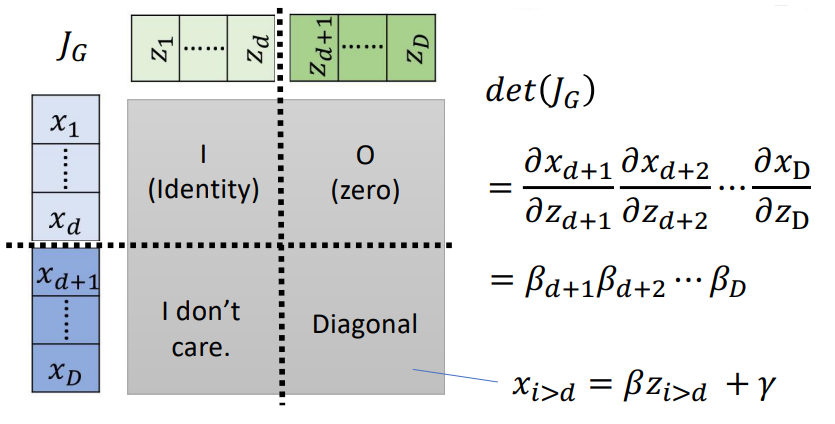
\includegraphics[height=0.9\textheight, width=\textwidth, keepaspectratio]{images/norm-flow/coupling_layer_3.png}
\end{figure}

\framebreak

\begin{figure}
    \centering
    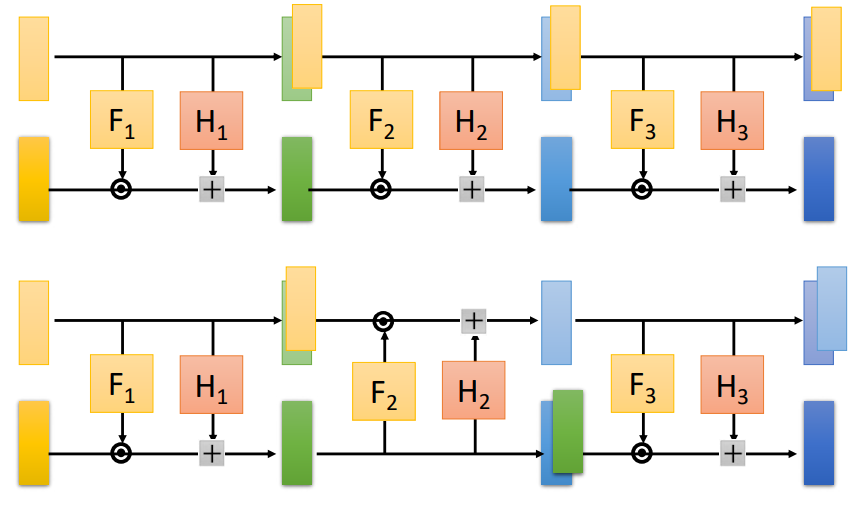
\includegraphics[height=0.9\textheight, width=\textwidth, keepaspectratio]{images/norm-flow/coupling_layer_4.png}
\end{figure}
    
\end{frame}